\subsubsection{Underdamped ($\Delta < 0$)}
This is probably the most complicated case.
Here, both roots are complex.
Specifically,
\begin{equation*}
	r = \frac{-b}{2m} \pm i\frac{\sqrt{\abs{\Delta}}}{2m}
\end{equation*}
Letting the coefficient of the imaginary part be $\omega$,
\begin{equation*}
	r = \frac{-b}{2m} \pm i\omega.
\end{equation*}
So, our solution becomes
\begin{equation*}
	y = e^{\frac{-b}{2m} t}\left(C_1\cos{(\omega t)} + C_2\sin{(\omega t)}\right).
\end{equation*}
Rewriting in terms of $\cos$ and a phase shift,
\begin{equation*}
	y = Ae^{\frac{-b}{2m} t}\cos{(\omega t - \phi)} \text{ where }
	A = \sqrt{A^2 + B^2} \text{, } \phi = \begin{cases}
		\arctan{\left(\frac{B}{A}\right)} + \pi & A \leq 0 \\
		\arctan{\left(\frac{B}{A}\right)} & A > 0
	\end{cases}.
\end{equation*}
\begin{center}
	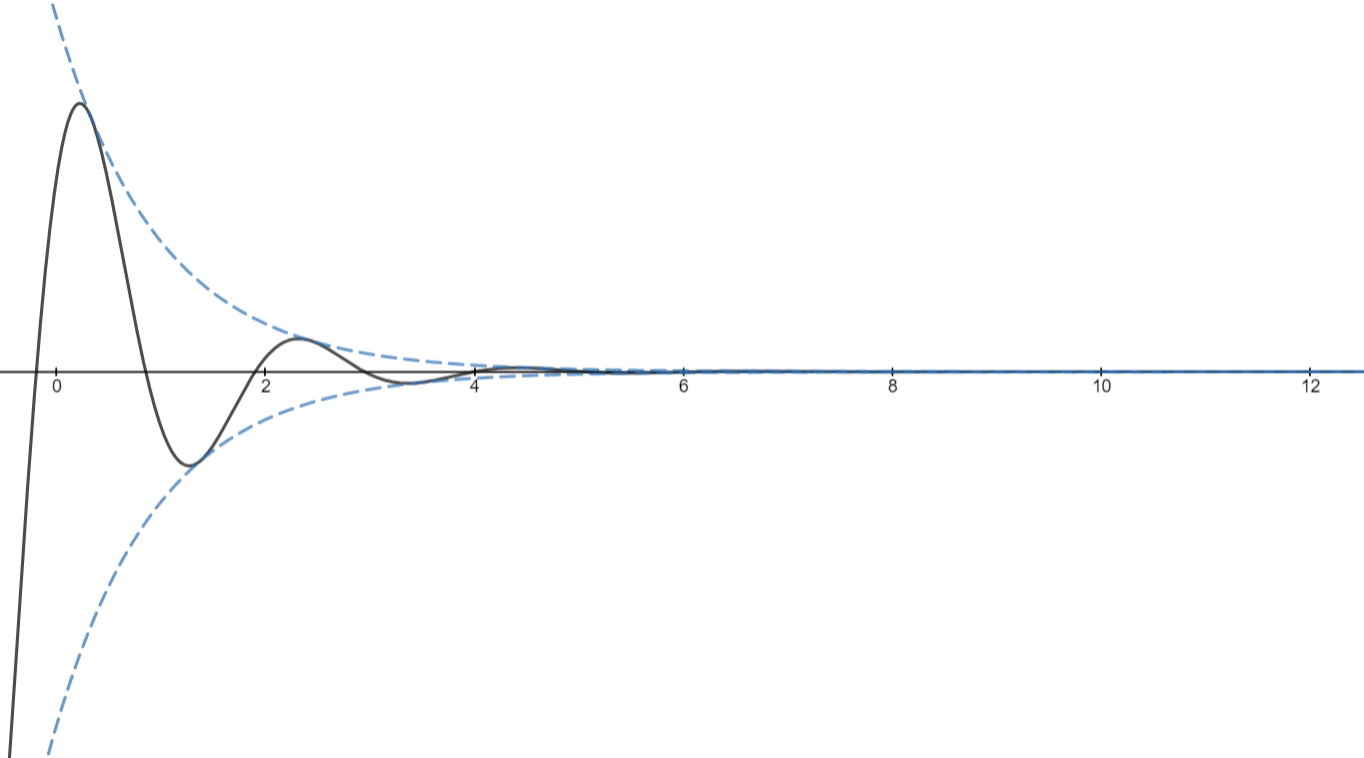
\includegraphics[width=0.5\textwidth]{./higherOrder/freeVibrs/underdamped.png}
\end{center}
Here, the exponential term dominates the limit, so
\begin{equation*}
	\lim\limits_{t \to 0}{Ae^{\frac{-b}{2m}t}\cos{(\omega t - \phi)}} = 0.
\end{equation*}
meaning the mass's oscillation decays over time, bounded by the exponential curves. 